\documentclass[border=1pt]{standalone}
\usepackage{tikz}
\usetikzlibrary{intersections,angles,quotes}

\begin{document}
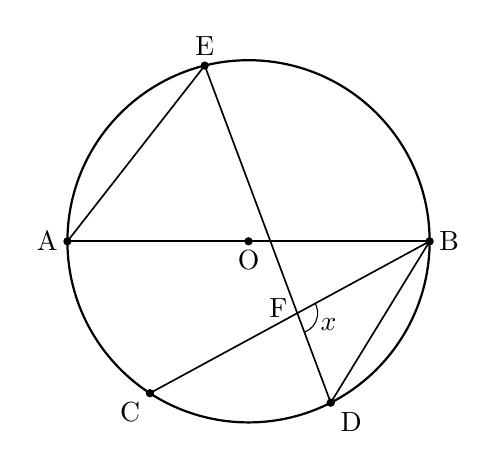
\begin{tikzpicture}

    % パラメータの定義
    \pgfmathsetmacro{\xmax}{4.6}
    \pgfmathsetmacro{\r}{\xmax/2}

    \pgfmathsetmacro{\thetaC}{237}
    \pgfmathsetmacro{\thetaD}{\thetaC+60}

    % 点の定義
    \coordinate (O) at (0,0);
    \coordinate (A) at (180:\r);
    \coordinate (B) at (0:\r);
    \coordinate (E) at (104:\r);
    \coordinate (C) at (\thetaC:\r);
    \coordinate (D) at (\thetaD:\r);
  
    % 円の描画
    \draw [thick] (O) circle (\r);

    % 線分の描画        
    \draw [semithick] (A) -- (B);
    \draw [semithick] (A) -- (E);
    \draw [semithick] (B) -- (D);
    \draw [semithick, name path=lineA] (B) -- (C);
    \draw [semithick, name path=lineB] (D) -- (E);

    % 点の描画
    \fill (O) circle (1.5pt) node[below] {$\mathrm{O}$};
    \fill (A) circle (1.5pt) node[left] {$\mathrm{A}$};
    \fill (B) circle (1.5pt) node[right] {$\mathrm{B}$};
    \fill (C) circle (1.5pt) node[below left] {$\mathrm{C}$};
    \fill (D) circle (1.5pt) node[below right] {$\mathrm{D}$};
    \fill (E) circle (1.5pt) node[above] {$\mathrm{E}$};

    % 交点F
    \node[name intersections={of=lineA and lineB, by=F}]
        at (F) [left, yshift=\xmax/2.5] {$\mathrm{F}$};
    
    % 角度の表示
    \draw pic["$x$", draw, angle eccentricity=\xmax/2.8, angle radius=1.6*\xmax] {angle=D--F--B};

\end{tikzpicture}
\end{document}
